\documentclass[8pt,xcolor=dvipsnames,xcolor=table]{beamer} 
%\usepackage{cite}
\mode<presentation> {
%\usetheme{CambridgeUS}
\usetheme{Madrid}
\usecolortheme[named=Mahogany]{structure}

%\usecolortheme{beaver}
\setbeamercovered{transparent}
%\usefonttheme[onlymath]{serif}
\usefonttheme{serif}
}
\usepackage{multirow}
\usepackage[english]{babel}
\usepackage[utf8]{inputenc}
\usepackage{times}
\usepackage{tikz}
\usepackage{subcaption} 
\usepackage{verbatim}
\usepackage{adjustbox}
\usepackage{tikz-feynman}
\usepackage{pgfplots}
\usepackage{tkz-fct}
%\usepackage{hyperref}
\usepackage{appendixnumberbeamer}

%%%%%%%%%%%%%%%%%%%%%%%%%%%
\title[ DY $Z'\rightarrow \tau\tau$] 
{Drell-Yan $Z'\rightarrow \tau\tau$}

\author[D. Barbosa (Universidad de los Andes)] 
{
Carlos Avila$^{1}$,  
\textbf{Diego Barbosa$^{1}$},
John Cumalat$^{2}$, 
Brenda Fabela Enriquez$^{4}$, \\
Andrés Flórez$^{1}$, 
Jorge Fraga$^{1}$, 
Alfredo Gurrola$^{4}$,  
Teruki Kamon$^{5}$ \\
Jose Ruiz$^{3}$,
Amal Sarkar, 
Nicolas Schonbeck$^{2}$,
Savanna Starko$^{4}$ \\
\medskip
{\footnotesize
Universidad de Los Andes$^{1}$ (CO)\\
 University of Colorado Boulder$^{2}$\\
 Universidad de Antioquia$^{3}$ (CO)\\
 Vanderbilt University$^{4}$\\
 Texas A\&M University$^{5}$ \\}
 \medskip
 {\large Workshop EXO}\\
 \medskip
 October 28, 2020 \\
 \medskip
\includegraphics[scale=0.5]{cernlogo.jpg} \qquad\qquad
\includegraphics[scale=0.35]{uniandes.png}
\includegraphics[scale=1.3]{colorado.png}
\includegraphics[scale=0.4]{antioquia.png}
\includegraphics[scale=0.4]{vanderbilt.jpg}
\includegraphics[scale=0.4]{tam.png} \qquad\qquad
\includegraphics[scale=0.11]{cmslogo}
}
%\institute[Universidad de los Andes]{}
\date{}

%------------------------------------------------
\begin{document}
%------------------------------------------------
\begin{frame}
\titlepage % Print the title page as the first slide
\end{frame}
%-------------------------------------------------------------------
\begin{frame}
\frametitle{Signal samples}

\begin{columns}

    \begin{column}{.45\textwidth}
    In this analysis we consider $Z'\rightarrow\tau_\mu\tau_h$, $Z'\rightarrow\tau_e\tau_h$ and $Z'\rightarrow\tau_h\tau_h$
    \begin{center}
    \includegraphics[width=0.8\linewidth]{EXO Non Hadronic Status Report 30/ztotautau.png}
    \end{center}
    \footnotesize
 The relevant parameters for the MC signal samples are:
 \begin{itemize}
    \item {\bf Masses:} 250, 500, 750, 1000, 1250, 1500, 1750, 2000, 2250, 2500, 2750, 3000, 3500, 4000 GeV.
    \item {\bf Couplings to light and heavy fermions} (\textcolor{blue}{$g_{l}=g_h$}): 0.1, 0.5, 1.0, 6.0,16. 
    \item {\bf  Coupling to vector bosons}: suppressed.
    %\item {\bf Input cards:} have been produced (param, proc, run): \href{https://www.dropbox.com/sh/up5099guxl5donz/AACRtbRFUzsMIbUd2wds1kANa?dl=0}{\textcolor{blue}{Find cards here}}
    \item \textcolor{blue}{ All the signal samples have been recently produced.}
\end{itemize}
\centering

\end{column}


      \begin{column}{.5\textwidth}

\centering

\includegraphics[width=0.83\linewidth]{EXO Non Hadronic Status Report 30/Mass_1500_gl_1.pdf}

\medskip

\includegraphics[width=0.845\linewidth]{EXO Non Hadronic Status Report 30/Mass_Zp_250GeV.pdf}

    \end{column}
    
  \end{columns}
%\centering
%\item All the signal samples are produced.

\end{frame}
%------------------------------------------------



%----------------------------------------------
\begin{frame}
\frametitle{Signal Region Selection Criteria for $Z'\rightarrow\tau_\ell\tau_h$}

The kinematic cuts used to obtain the control regions for $Z'\rightarrow\tau_\ell\tau_h$ are listed below:
%\begin{itemize}
 %   \item Event selection optimized to maximize significance.
  %  \item MC and data samples are listed in the following slide: \hyperlink{appA}{\beamerbutton{Appendix A}}
   % \item In order to search for $Z'$ signature, we use  $m_{reco}(\ell,\tau,\Delta{p_{T}}(\ell,\tau))$.
%\end{itemize}
\\
\medskip

\small
\begin{tabular}{ll}
\hline
Trigger ($\tau_{\mu}\tau_{h}$) & HLT\_IsoMu24 (2016),  HLT\_IsoMu27 (2017,2018) \\
Trigger ($\tau_{e}\tau_{h}$) & HLT\_Ele27\_WPTight\_Gsf (2016),  HLT\_Ele35\_WPTight\_Gsf (2017,2018)  \\
\hline
\end{tabular}
\begin{columns}
    \begin{column}{.6\textwidth}
\centering
\resizebox{0.9\textwidth}{!}{
\begin{tabular}{lll}

$\ell = \mu $ or e & $N(\ell)$ 			& $= 1$  \\
& ID                            & Tight \\
& $p_T(\mu/e)$			& (35/55) GeV  \\
& $|\eta(\ell)|$ 		& $<2.1$   \\
& Relative Isolation ($\mu$) 	& $<0.15$ \\
\hline 
Tau & $N(\tau_h)$ 			& $= 1$  \\
& $p_T(\tau_h)$			& $>20$ GeV   \\
& $|\eta(\tau_h)|$ 	& $<2.1$   \\
& DeepTauID Isolation* 			& Tight \\
& Prongs 			& 1 or 3 hp \\
%& Discriminator against $\mu$   & Tight \\
%& Discriminator against $e$     & Tight \\
\hline
$\ell-\tau$ pair & $Q(\ell)Q(\tau)$ 	& $<0$ (OS)  	\\
& \textcolor{blue}{$\cos\Delta\phi(\ell,\tau_h)$} &$<-0.98$ \\
\hline
b-jets$^{**}$ & $N(b\text{-jets})$ & $=0$\\
\hline
leading $\ell$ & \textcolor{blue}{ $\cos\Delta\phi(p_T^{\text{lead-}\ell},E_T^{miss})$} & $<-0.95$ \\
&\textcolor{blue}{ $m_T(p_T^{\text{lead-}\ell},E_T^{miss})$} & $>150$ GeV \\
\hline
Dijet veto & $N(jet^{\dagger} pairs)$ passing VBF$^{\ddag}$ & =0 \\
\hline  
\end{tabular}
}
    \end{column}
    \begin{column}{.45\textwidth}
\includegraphics[width=0.9\textwidth]{ztomu.png}

\textcolor{red}{Orthogonal to the VBF $Z'$ analysis}
    \end{column}
\end{columns}
 \medskip
\footnotesize
$^{*}$TauIDAlgorithm: Tau\_idDeepTau2017v2p1

$^{**}$b-jet: $p_T>30$, $|\eta|<2.4$ GeV with CSV medium (2016), DeepCSV tight (2017), DeepF tight (2018)

$^{\dagger}$Jets: $p_T>30$, $|\eta|<5$ GeV with Loose ID (2016), Tight ID (2017,2018)

$^{\ddag}$VBF events: $|\eta(jj)|<3.8$, $m(jj)>300$ GeV
%* sample-dependent PU corrections (2017)

\end{frame}
%------------------------------------------------

%----------------------------------------------
%------------------------------------------------
\begin{frame}
\frametitle{$t\bar{t}$ Control Regions for  $Z'\rightarrow\tau_\mu\tau_h$ and  $Z'\rightarrow\tau_e\tau_h$ }

\begin{itemize}
\item To obtain the $t\bar{t}$ CR we require $N(b\text{-jets}) \ge 1$. 
\item The $t\bar{t}$ distributions for $\tau_\mu\tau_h$ (left) and $\tau_e\tau_h$ (center and right) have the scale factor applied.
\end{itemize}
  
\begin{columns}
\begin{column}{.33\textwidth}
\centering
\includegraphics[width=\textwidth]{muTau_ttbarCR_2016.pdf}
\small
\resizebox{0.7\textwidth}{!}{
\begin{tabular}{lcr}
\hline\hline
Process   & Events (2016)           \\
\hline
W+jets    & 0.0$\pm$0.0 \\
Drell-Yan & 16.5$\pm$4.9 \\
$t\bar{t}$    & 231.1$\pm$8.6 \\
SingleTop & 24.9$\pm$2.1 \\
Diboson   & 2.9$\pm$0.6 \\
\hline
TotalBack.& 275.5$\pm$10.2 \\
Data      & 285       \\
\hline
Purity & 84\%   \\
\hline
Scale Factor & 1.04 $\pm$0.10   \\
\hline\hline
\end{tabular}
}
\end{column}


\begin{column}{.32\textwidth}
\centering
\includegraphics[width=\textwidth]{EXO Non Hadronic Status Report 30/plots_eTau_2017_PlotsN_ttbar2017-ETau-RecMass.pdf}
\small
\resizebox{0.7\textwidth}{!}{
\begin{tabular}{lcr}
\hline\hline
Process   & Events (2017)           \\
\hline
W+jets    &  0.5 $\pm$ 0.3\\
Drell-Yan & 0.4 $\pm$ 0.1\\
ttbar     & 225.4 $\pm$ 9.4 \\
SingleTop & 23.3 $\pm$ 2.1 \\
Diboson   & 0.5 $\pm$ 0.3  \\
\hline
Total Back.& 250.1 $\pm$ 9.6 \\
Data      & 253       \\
\hline
Purity & 90\%   \\
\hline
Scale Factor & 1.01 $\pm$0.09   \\
\hline\hline
\end{tabular}
}
\end{column}

\begin{column}{.315\textwidth}
\centering
\includegraphics[width=\textwidth]{EXO Non Hadronic Status Report 30/etau_2018_ttbarRecMass.pdf}
\small
\resizebox{0.7\textwidth}{!}{
\begin{tabular}{lcr}
\hline\hline
Process   & Events (2018)             \\
\hline
W+jets    & 2.2 $\pm$ 1.5 \\
Drell-Yan & 1.2 $\pm$ 0.3 \\
ttbar     & 436.5 $\pm$ 6.0 \\
SingleTop & 41.0 $\pm$ 3.3 \\
Diboson   & 0.7 $\pm$ 0.2 \\
\hline
Total Back.& 481.6$\pm$ 7.0 \\
Data      & 429      \\
\hline
Purity & 91\%   \\
\hline
Scale Factor & 0.88 $\pm$0.07  \\
\hline\hline
\end{tabular}
}
\end{column}
\end{columns}
 \centering
 
 \textcolor{blue}{\boxed{$$N_{SR}^{t\bar{t}}=SF\cdot N_{SR}^{MC}$$}}
\end{frame}
%------------------------------------------------
%-----------------------------------------------
%------------------------------------------------
\begin{frame}
\frametitle{Drell-Yan Control Regions for $Z'\rightarrow\tau_e\tau_h$ and $Z'\rightarrow\tau_\mu\tau_h$ }
To obtain the Drell-Yan CR for the $\tau_l\tau_h$ channels we require the following cuts:
\begin{center}
\small
\resizebox{0.3\textwidth}{!}{
\begin{tabular}{l}
\hline
%Only for 2016 \\
\hline
$m_T(p_T^{\text{lead-}\ell},E_T^{miss})<150$ GeV \\
$70<m_{rec}(\ell,\tau_h,\Delta p_T)<110$ GeV  \\
%$N_{SR}^{DY}=SF\cdot N_{SR}^{MC}$
\hline
\end{tabular} }
\end{center}
\begin{columns}
\begin{column}{.34\textwidth}
%\centering
%$\tau_e\tau_h$
%\begin{center}
%\small
%\resizebox{0.8\textwidth}{!}{
%\begin{tabular}{l}
%\hline
%Only for 2016 \\
%\hline
%$m_T(p_T^{\text{lead-}\ell},E_T^{miss})<150$ GeV \\
%$70<m_{rec}(e,\tau_h,\Delta p_T)<110$ GeV  \\
%\hline
%\end{tabular} }

%\end{center}
\centering
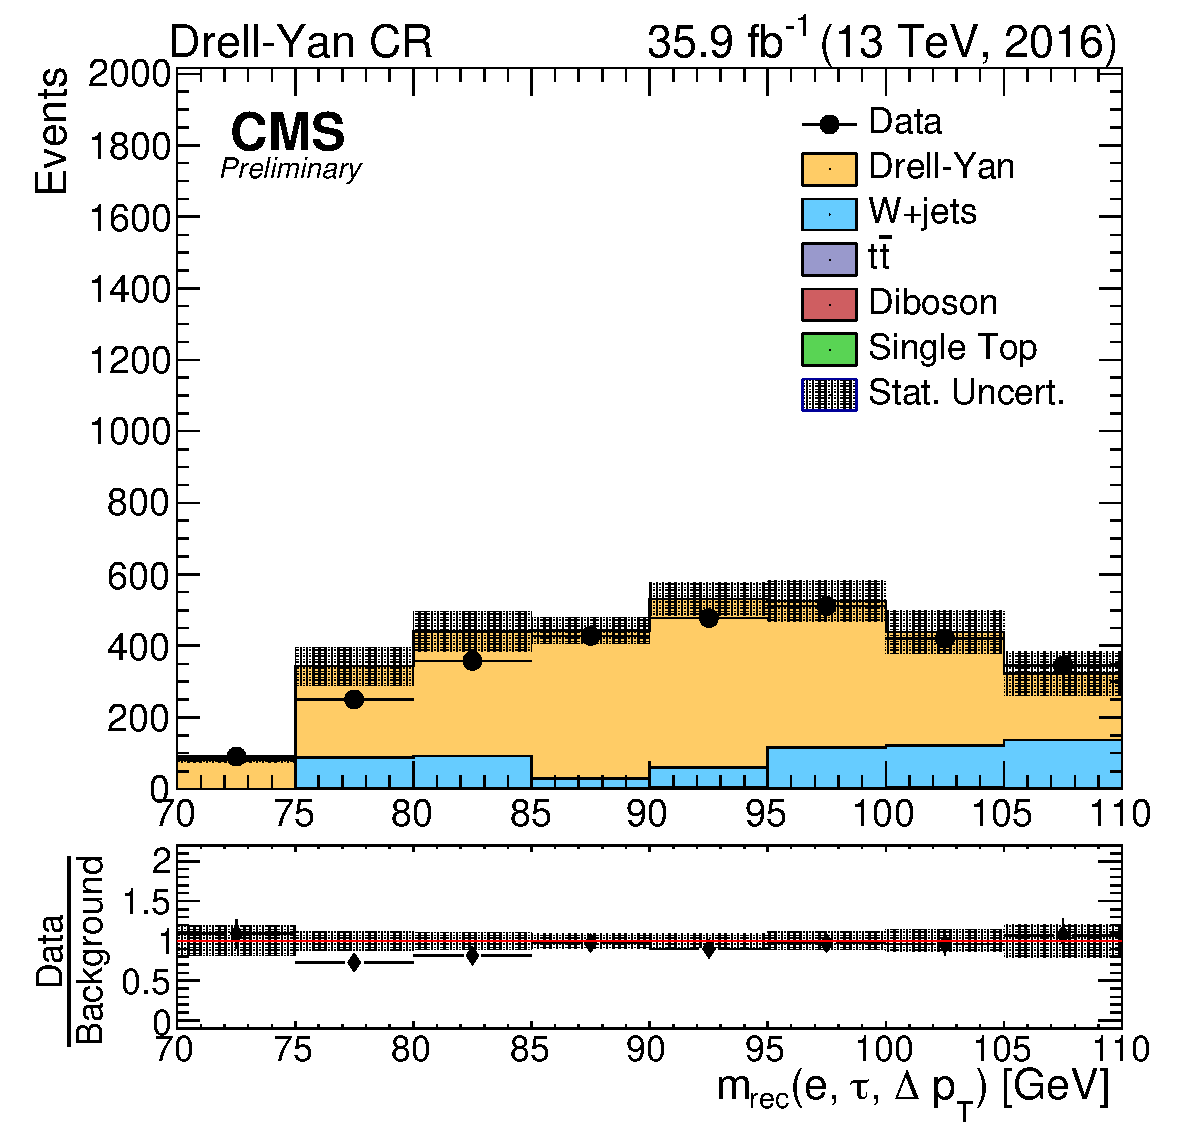
\includegraphics[width=0.88\textwidth]{EXO Non Hadronic Status Report 30/DY2016_etau_recMass.pdf}
\small
\resizebox{0.85\textwidth}{!}{
\begin{tabular}{lcr}
\hline\hline
Process   & Events (2016)             \\
\hline
W+jets    & 626.4 $\pm$ 123.0 \\
Drell-Yan &  2388.3 $\pm$ 59.3 \\
ttbar     & 5.7 $\pm$ 1.5 \\
SingleTop & 1.3 $\pm$ 0.5 \\
Diboson   &  10.0 $\pm$ 1.3 \\
\hline
Total Back.& 3031.7 $\pm$ 136.6 \\
Data      & 2892      \\
\hline
Purity & 79\%   \\
\hline
Scale Factor & 0.94 $\pm$0.07   \\
\hline\hline
\end{tabular}
}
\end{column}



\begin{column}{.33\textwidth}
%\centering
%$\tau_\mu\tau_h$
%\begin{center}
%\small
%\resizebox{0.8\textwidth}{!}{
%\begin{tabular}{l}
%\hline
%For 2017. \\
%\hline
%$m_T(p_T^{\text{lead-}\ell},E_T^{miss})<150$ GeV \\
%$70<m_{rec}(\mu,\tau_h,\Delta p_T)<110$ GeV  \\
%\hline
%\end{tabular}} 

%\end{center}
\includegraphics[width=0.88\textwidth]{muTau_dyCR_2017.pdf}
\small
\resizebox{0.85\textwidth}{!}{
\begin{tabular}{lcr}
\hline\hline
Process   & Events   (2017)          \\
\hline
W+jets    & 846.1$\pm$180.8 \\
Drell-Yan & 3526.1$\pm$100.0 \\
$t\bar{t}$    & 16.5$\pm$1.0 \\
SingleTop & 3.2$\pm$0.8 \\
Diboson   & 21.5$\pm$2.2 \\
\hline
TotalBack.& 4413.5$\pm$206.7 \\
Data      & 4077       \\
\hline
Purity & 80\%   \\
\hline
Scale Factor & 0.90 $\pm$0.07   \\
\hline\hline
\end{tabular}
}
\end{column}


\begin{column}{.33\textwidth}
%\centering
%$\tau_\mu\tau_h$
%\begin{center}
%\small
%\resizebox{0.8\textwidth}{!}{
%\begin{tabular}{l}
%\hline
%For 2018. \\
%\hline
%$m_T(p_T^{\text{lead-}\ell},E_T^{miss})<150$ GeV \\
%$70<m_{rec}(\mu,\tau_h,\Delta p_T)<110$ GeV  \\
%\hline
%\end{tabular}} 

%\end{center}

\includegraphics[width=0.90\textwidth]{muTau_dyCR_2018.pdf}
\small
\resizebox{0.85\textwidth}{!}{
\begin{tabular}{lcr}
\hline\hline
Process   & Events   (2018)          \\
\hline
W+jets    & 1015.6$\pm$240.1 \\
Drell-Yan & 5586.6$\pm$147.8 \\
$t\bar{t}$    & 22.0$\pm$1.5 \\
SingleTop & 5.8$\pm$1.2 \\
Diboson   & 24.2$\pm$1.5 \\
\hline
TotalBack.& 6654.2$\pm$281.9 \\
Data      & 5600       \\
\hline
Purity & 84\%   \\
\hline
Scale Factor & 0.81 $\pm$0.06   \\
\hline\hline
\end{tabular}
}
\end{column}
\end{columns}
\begin{itemize}
    \small
    \item \textcolor{red}{For 2017 and 2018 for the $\tau_e\tau_h$ channel we cannot obtain a DY CR since $p_T(e)>55$ GeV}.
\end{itemize}
\end{frame}
%------------------------------------------------

%------------------------------------------------
\begin{frame}
\frametitle{QCD Estimation Strategy for $Z'\rightarrow\tau_\mu\tau_h$ and  $Z'\rightarrow\tau_e\tau_h$}
We estimate QCD in a  data-driven way for the $\tau_l\tau_h$ channels using the ABCD method.
\begin{columns}
    \begin{column}{.45\textwidth}

 \centering{
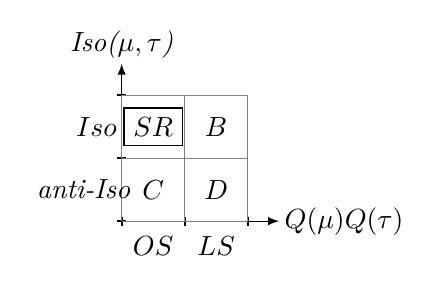
\begin{tikzpicture}[scale=0.8]
\tkzInit[xmin=0,xmax=10,
         ymin=0,ymax=10,
         xstep=5,ystep=5]
\tkzDrawX[label={\textit{$Q(\mu)Q(\tau)$}}, right=1pt]
\tkzDrawY[label={\textit{Iso($\mu,\tau$)}},above=1pt]
\tkzGrid(0,0)(10,10) 
\tkzText(2.5,-2){$OS$}
\tkzText(7.5,-2){$LS$}
\tkzText(-2,7.5){$Iso$}
\tkzText(-3,2.5){\textit{anti-Iso}}
\tkzText[draw](2.5,7.5){$SR$}
\tkzText(7.5,7.5){$B$}
\tkzText(2.5,2.5){$C$}
\tkzText(7.5,2.5){$D$}
%\tkzFct[domain=0:2,color=blue, thick,-]{1}
\end{tikzpicture}
}

    \end{column}
    \begin{column}{.45\textwidth}
    
   
\begin{center}
\footnotesize
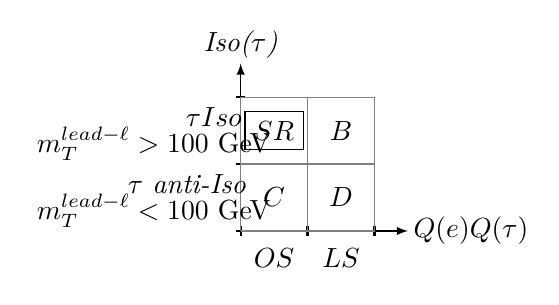
\begin{tikzpicture}[scale=0.85]
\tkzInit[xmin=0,xmax=10,
         ymin=0,ymax=10,
         xstep=5,ystep=5]
\tkzDrawX[label={\textit{$Q(e)Q(\tau)$}}, right=1pt]
\tkzDrawY[label={\textit{Iso($\tau$)}},above=1pt]
\tkzGrid(0,0)(10,10) 
\tkzText(2.5,-2){$OS$}
\tkzText(7.5,-2){$LS$}
\tkzText(-2,8.5){$\tau Iso$}
\tkzText(-6.5,6.5){$m_T^{\text{lead-}\ell}>100$ GeV}
\tkzText(-4,3.5){$\tau$ \textit{anti-Iso}}
\tkzText(-6.5,1.5){$m_T^{\text{lead-}\ell}<100$ GeV}
\tkzText[draw](2.5,7.5){$SR$}
\tkzText(7.5,7.5){$B$}
\tkzText(2.5,2.5){$C$}
\tkzText(7.5,2.5){$D$}
%\tkzFct[domain=0:2,color=blue, thick,-]{1}
\end{tikzpicture}


%\includegraphics[width=0.75\linewidth]{Plot1Mrec.pdf}   
\end{center}   

 \end{column}
 \end{columns}
 
 \begin{equation*}
\textcolor{blue}{
\boxed{N_{SR}^{QCD}&=R_{OS/LS}\cdot(N_{B}^{\text{Data}}-N_{B}^{\text{non-QCD MC}})_{LS} }}
   \quad\text{where }\quad 
\textcolor{blue}{
\boxed{R_{OS/LS}=\frac{(N_{C}^{\text{Data}}-N_{C}^{\text{non-QCD MC}})_{OS}}
{(N_{D}^{\text{Data}}-N_{D}^{\text{non-QCD MC}})_{LS}}}}
\end{equation*}
 
 %\begin{center}
  %   $N_{SR}^{QCD}&=R_{OS/LS}\cdot(N_{B}^{\text{Data}}-N_{B}^{\tex%t{non-QCD MC}})_{LS} $  $$\boxed{R_{OS/LS}=
%\frac{(N_{C}^{\text{Data}}-N_{C}^{\text{non-QCD MC}})_{OS}}
%{(N_{D}^{\text{Data}}-N_{D}^{\text{non-QCD MC}})_{LS}}}$$
% \end{center}

\begin{columns}
%\begin{column}{.25\textwidth}
%\centering
%\includegraphics[width=\textwidth]{muTau_ratio_QCDs_2016.pdf}
%\end{column}

\begin{column}{.5\textwidth}
\centering
\includegraphics[width=0.73\textwidth]{EXO Non Hadronic Status Report 30/muTau_ratio_QCDs_2016.pdf}
\end{column}

\begin{column}{.5\textwidth}
\centering
\includegraphics[width=0.78\textwidth]{EXO Non Hadronic Status Report 30/etau_QCD_RatioPlot2017.pdf}
\end{column}
\end{columns}
%\small{
%\item \textcolor{red}{
%QCD estimation done for the $\tau_\mu\tau_h$ channel for the three years. For the $\tau_e\tau_h$ channel is ongoing and close to being completed for 2018.}}

\end{frame}
%------------------------------------------------
%------------------------------------------------
\begin{frame}
\frametitle{W+jets Control Region for $Z'\rightarrow\tau_\mu\tau_h$}
Using the following kinematic cuts a control region for W+Jets has been obtained :
\begin{center}
\begin{tabular}{l}
\hline
$m_T(p_T^{\text{lead-}\ell},E_T^{miss})<150$ GeV\\
$m_{rec}(\mu,\tau_h,\Delta p_T)<250$ GeV \\
$\tau$ anti-Isolation\\
\hline
\end{tabular}    
\end{center}
\begin{columns}
\begin{column}{.33\textwidth}
\centering
\includegraphics[width=\textwidth]{muTau_WjetsCR_QCD_2016.pdf}
\small
\resizebox{0.8\textwidth}{!}{
\begin{tabular}{lcr}
\hline\hline
Process   & Events (2016)            \\

\hline
Purity & 63\%   \\
\hline
Scale Factor & 0.88 $\pm$0.05   \\
\hline\hline
\end{tabular}
}
\end{column}
\begin{column}{.33\textwidth}
\centering
\includegraphics[width=\textwidth]{muTau_WjetsCR_QCD_2017.pdf}
\small
\resizebox{0.8\textwidth}{!}{
\begin{tabular}{lcr}
\hline\hline
Process   & Events (2017)            \\
\hline
Purity & 70\%   \\
\hline
Scale Factor & 0.98 $\pm$0.06   \\
\hline\hline
\end{tabular}
}
\end{column}
\begin{column}{.33\textwidth}
\centering
\includegraphics[width=\textwidth]{EXO Non Hadronic Status Report 30/muTau_WjetsCR_QCD_2018-2.pdf}
\small
\resizebox{0.8\textwidth}{!}{
\begin{tabular}{lcr}
\hline\hline
Process   & Events  (2018)           \\
\hline
Purity & 73\%   \\
\hline
Scale Factor & 0.96 $\pm$0.05   \\
\hline\hline
\end{tabular}
}
\end{column}
\end{columns}
\smallskip
\smallskip
\centering
 \textcolor{blue}{\boxed{$$N_{SR}^{W+Jets}=SF\cdot N_{SR}^{MC}$$}}
\end{frame}

%------------------------------------------------

\begin{frame}
\frametitle{Signal Region Selection Criteria for $Z'\rightarrow\tau_h\tau_h$}


\small

\begin{columns}


    \begin{column}{.5\textwidth}
    
\includegraphics[width=0.6\textwidth]{ztotaus.png}
\centering
\resizebox{0.9\textwidth}{!}{
\begin{tabular}{lll}
\hline
Trigger ($\tau_{h}\tau_{h}$) & HLT\_DoubleMediumIsoPFTau \\
\hline
Tau & $N(\tau_h,\tau_h)$ 			& $\geq 1$  \\
& $N(\tau_h)$ 			& $= 2$  \\
& $p_T(\tau_h)$			& $>70$ GeV   \\
& $|\eta(\tau_h)|$ 	& $<2.1$   \\
& DeepTauID Isolation$^*$ 			& Tight \\
& Prongs 			& 1 or 2 or 3 hp \\
& $Q(\tau_1)Q(\tau_2)$ 	& $<0$ (OS)  	\\
\hline
b-jets$^{**}$ & $N(b\text{-jets})$ & $=0$\\
\hline
Topological &\textcolor{blue}{$\cos\Delta\phi(\tau_1,\tau_2)$} & $<-0.95$ \\
Selections &\textcolor{blue}{$|\cos\Delta\phi(p_T^{\text{lead-}\tau},E_T^{miss})|$} & $>0.90$ \\
& \textcolor{blue}{$E_T^{miss}$} & $>30$ GeV \\
\hline
%Dijet veto & $N(jet^{\dagger} pairs)$ passing VBF$^{\ddag}$ & =0 \\
%\hline  
\end{tabular}
}

\item \textcolor{red}{
Drell-Yan control region cuts:}
\\
\medskip
\centering
            \begin{tabular}{ l l }
                \hline\hline
                Baseline Cuts & Value \\ 
                \hline
                %$N(\tau\tau)$               & = 1 \\
                $N(\tau)$                   & =2 \\ 
                %$|\eta(\tau)|$                & $< 2.1$ \\ 
                %$p_{T}(\tau)$               & $\geq 70$ GeV \\ 
                $m(\tau,\tau)$              & [0, 100] GeV \\
                %\hline\hline
                %Topological Selections      & Value \\
                \hline
                $E^{miss}_{T}$              & $< 30$ GeV \\
                \hline\hline
            \end{tabular}
    \end{column}
    \begin{column}{.5\textwidth}
    
\textcolor{blue}{Reconstructed invariant mass for 2016.}
\centering
\includegraphics[width=0.99\linewidth]{EXO Non Hadronic Status Report 30/diTau_dyCR2016_ditaurecomassdeltapt_101420.pdf}
            

\textcolor{blue}{Reconstructed invariant mass for 2018.}
\includegraphics[width=0.99\linewidth]{EXO Non Hadronic Status Report 30/diTau_dyCR2018_ditaurecomassdeltapt_100720.pdf}

    \end{column}
\end{columns}
 

\end{frame}
%------------------------------------------------
\begin{frame}
\frametitle{QCD Data-Driven Estimation Strategy for $Z'\rightarrow\tau_h\tau_h$}

\begin{columns}
    \begin{column}{.45\textwidth}
We estimate QCD in a  data-driven way for the $\tau_h\tau_h$ channel using the ABCD method.

\centering{
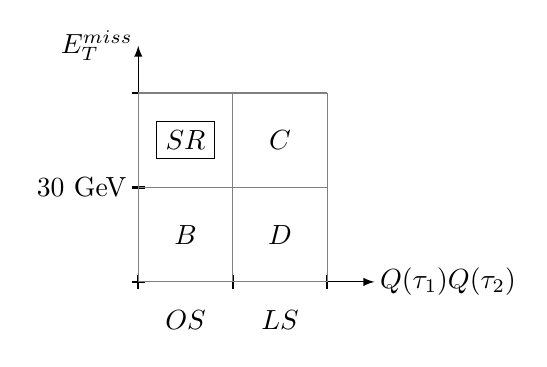
\begin{tikzpicture}[scale=1.2]
\tkzInit[xmin=0,xmax=10,
         ymin=0,ymax=10,
         xstep=5,ystep=5]
\tkzDrawX[label={\textit{$Q(\tau_1)Q(\tau_2)$}}, right=1pt]
\tkzDrawY[label={$E_T^{miss}$},left=1pt]
\tkzGrid(0,0)(10,10) 
\tkzText(2.5,-2){$OS$}
\tkzText(7.5,-2){$LS$}
\tkzText(-3,5){30 GeV}
\tkzText[draw](2.5,7.5){$SR$}
\tkzText(7.5,7.5){$C$}
\tkzText(2.5,2.5){$B$}
\tkzText(7.5,2.5){$D$}
%\tkzFct[domain=0:2,color=blue, thick,-]{1}
\end{tikzpicture}

 \begin{center}
     $N_{SR}^{QCD}&=R_{OS/LS}\cdot(N_{B}^{\text{Data}}-N_{B}^{\text{non-QCD MC}})_{LS} $
 \end{center}

The transfer factor ($R_{OS/LS}$) from LS to OS CRs is defined as
$$\boxed{R_{OS/LS}=
\frac{(N_{B}^{\text{Data}}-N_{B}^{\text{non-QCD MC}})_{OS}}
{(N_{D}^{\text{Data}}-N_{D}^{\text{non-QCD MC}})_{LS}}}$$


}
\end{column}


      \begin{column}{.5\textwidth}

\centering
%\includegraphics[width=0.8\linewidth]{EXO Non Hadronic Status Report 30/2018 m_reco CR_B inverted (flipped) iso (Savanna).pdf}
            

\includegraphics[width=0.9\linewidth]{EXO Non Hadronic Status Report 30/2018 m_reco CR_D inverted (flipped) iso (Savanna).pdf}

\includegraphics[width=0.8\linewidth]{EXO Non Hadronic Status Report 30/2018_ATF_Draft_3.pdf}

    \end{column}
    
  \end{columns}
\centering
\item \textcolor{red}{QCD data-driven estimation done for the three years.}  

\end{frame}
%------------------------------------------------
\section{Summary and Work Plan}
%------------------------------------------------
\begin{frame}
\frametitle{Summary}
\Large{
\begin{itemize}
    \item We have optimized our selection criteria for best signal significance.
    \item \textbf{We have implemented the DeepTau ID algorithm as requested.}
    \item \textbf{The background estimation for all channels is 90$\%$ completed.}
    \item The work on the three different channels has been documented in the analysis note AN-20-134 \href{https://gitlab.cern.ch/tdr/notes/AN-20-134/-/blob/master/AN-20-134_temp.pdf}{\textcolor{blue}{\underline{(AN-20-134  link here)}}} and it had been sent to the conveners.
    \item We have a dedicated Twiki page for the analysis. \href{https://twiki.cern.ch/twiki/bin/viewauth/CMS/EXODYZprimeTauTau20134}{\textcolor{blue}{\underline{(Twiki link here)}}}
    \item \textbf{All the signal samples were produced.}
    \item We expect to converge with the analysis in the next couple of months.
    
\end{itemize}
}
\end{frame}
%------------------------------------------------
\appendix
\section{Appendix}
\begin{frame}
\centering
\Huge
Backup Slides
\end{frame}
%------------------------------------------------
\begin{frame}
\frametitle{QCD  for $Z'\rightarrow\tau_\mu\tau_h$ and  $Z'\rightarrow\tau_e\tau_h$- Transfer Factors}
\begin{columns}
    \begin{column}{.50\textwidth}
    \centering
    $\tau_\mu\tau_h$
    
\begin{figure}
  \begin{subfigure}[b]{0.4\textwidth}
    \includegraphics[width=\textwidth]{muTau_QCD_CRC_2016.pdf}
    \caption{CR-C}
    \label{fig:1}
  \end{subfigure}
  %
  \begin{subfigure}[b]{0.4\textwidth}
    \includegraphics[width=\textwidth]{muTau_QCD_CRD_2016.pdf}
    \caption{CR-D}
    \label{fig:2}
  \end{subfigure}
\end{figure}    
    
\centering
\resizebox{0.8\textwidth}{!}{
\begin{tabular}{lccc}
\hline\hline
CR   & Events & Background & QCD Purity             \\
\hline
B &   392 & 17.7 $\pm$ 6.4 & 95$\%$ \\
C &   352 &  37.6 $\pm$ 27.8 & 89$\%$ \\
D &   211 & 48.6$\pm $34.8   & 78$\%$ \\
\hline\hline
\end{tabular} 
}
\begin{itemize}


\item The transfer factor obtained for the $\tau_\mu\tau_h$ is
\end{itemize}
\begin{equation*}

R_{OS/LS}=
\frac{N_{C,OS}^{QCD}}{N_{D,LS}^{QCD}}
=1.44\pm 0.19
\end{equation*}   

    \end{column}
    
    
    \begin{column}{.50\textwidth}
     \centering
    $\tau_e\tau_h$
\begin{figure}
  \begin{subfigure}[b]{0.4\textwidth}
    \includegraphics[width=\textwidth]{EXO Non Hadronic Status Report 30/plots_eTau_2016_PlotsN_QCD2016-OS-M160.pdf}
    \caption{CR-C}
    \label{fig:1}
  \end{subfigure}
  %
  \begin{subfigure}[b]{0.4\textwidth}
    \includegraphics[width=\textwidth]{EXO Non Hadronic Status Report 30/plots_eTau_2016_PlotsN_QCD2016-LS-M160.pdf}
    \caption{CR-D}
    \label{fig:2}
  \end{subfigure}
\end{figure}    
    
\centering
\resizebox{0.8\textwidth}{!}{
\begin{tabular}{lccc}
\hline\hline
CR   & Events & Background & QCD Purity             \\
\hline
B &   1357 & 662.3 $\pm$ 105.0 & 51$\%$ \\
C & 3684&  2191.2 $\pm$ 184.5 & 41$\%$ \\
D & 2143& 724$\pm $116.1   & 62$\%$ \\
\hline\hline
\end{tabular} 
}

\begin{itemize}


\item The transfer factor obtained for the $\tau_e\tau_h$ is
\end{itemize}
\begin{equation*}

R_{OS/LS}=
\frac{N_{C,OS}^{QCD}}{N_{D,LS}^{QCD}}
=1.10\pm 0.18
\end{equation*}   

    \end{column}
  \end{columns}


\end{frame}



\end{document} 